\documentclass[hyperref={pdfpagemode=FullScreen, colorlinks=false}]{beamer}

\usepackage{selinput}			% Inputencoding
	\SelectInputMappings{adieresis={ä}, germandbls={ß}, Euro={€}}
\usepackage[T1]{fontenc}		% Fontencoding
%
\usepackage{pifont}
\usepackage{csquotes,siunitx}			% Anführungszeichen; wird von biblatex gewünscht
\usepackage[backend=biber,citestyle=alphabetic,uniquelist=false]{biblatex}	% Literatur formatieren
\addbibresource{bodendynamik.bib}	% Literaturdatenbank
\usepackage{caption} 
\usepackage{subfig}
\usepackage{comment}
%%%%%%%%%%%%%%%%%%%%%%%%%%%%%%%%%%%%%%%%%%%%%%%%%%%%%%%%%%%%%%%%%%%%%%%%%%%%%%%%%%%%%%%%%%%%%%%%%%%%%%%
% Thema für Präsentation
\usetheme[fusszeile=ernstcolor,sprache=ngerman,seite=letzte,
verhaeltnis=16:10,
hausschrift=false,
navigation=false,
titelseite=blau]{TUBAF}

\TUBAFZweitlogo{
\includegraphics{fig_pdf/UFZ_logo_inv.pdf}}

%%%%%%%%%%%%%%%%%%%%%%%%%%%%%%%%%%%%%%%%%%%%%%%%%%%%%%%%%%%%%%%%%%%%%%%%%%%%%%%%%%%%%%%%%%%%%%%%%%%%%%%
% Optionen für Anmerkungen
\mode<presentation>{%
\setbeameroption{hide notes}				% keine Notizen (default)
%\setbeameroption{show notes}				% Notizen und Frames gemischt
%\setbeameroption{show only notes}			% nur Notizen
%
%\usepackage{pgfpages}					% wird für nachfolgendes benötigt
%\setbeameroption{show notes on second screen=left}	% wie gesagt; left, right, bottom, top
}




%%% DK packages and settings
\usepackage{amsmath}
\usepackage{pgfpages}
\pgfpagesuselayout{resize to}[a4paper, landscape]   % border shrink=5mm
\usepackage{siunitx}  
%\sisetup{locale = DE} 
\usepackage{tikz}
\usepackage{pgfplots}
\usepackage{animate}

\usetikzlibrary{math}
%\usetikzlibrary{datavisualization.formats.functions}
%\usetikzlibrary{datavisualization}
\usetikzlibrary{intersections}
\usepgfplotslibrary{groupplots,dateplot}
\pgfplotsset{compat=1.16}

\tikzset{
%DKspring(length) length=2...10
DKspring/.pic={
\coordinate (half_up) at (0.5*0.125*#1-0.5*0.125*2, 0.5*0.125*10-0.5*0.125*#1); %at (0.5*(#1-0.2), 0.5*(1.0-#1));
\coordinate (full_up)   at ( 0.125*#1-    0.125*2,     0.125*10-    0.125*#1);
\coordinate (full_down) at ( 0.125*#1-    0.125*2,    -0.125*10+    0.125*#1);
\draw (0, 0) -- ++(1, 0) -- ++(half_up)
    -- ++(full_down) -- ++(full_up) 
    -- ++(full_down) -- ++(full_up)
    -- ++(full_down) -- ++(full_up)
    -- ++(full_down) -- ++(half_up)
    -- ++(1, 0);
    },   
%DKdashpot(length) length=02...10    
DKdashpot/.pic={
\coordinate (upper_end) at (#1-0.5, 0.5);
\coordinate (lower_end) at (#1-0.5,-0.5);
\coordinate (upper_pos) at (#1-1, 0.5);
\coordinate (lower_pos) at (#1-1,-0.5);
\coordinate (center_pos) at (#1-1, 0.0);
\coordinate (center_end) at (#1, 0.0);
\draw (0, 0) -- ++(1, 0);
\draw (upper_end) -- (1, 0.5) -- (1, -0.5) -- (lower_end);
\draw (center_pos) -- (center_end);
\draw (upper_pos) -- (lower_pos);
    },
DKbase/.pic={
\draw[thick] (0, 1.5) -- (0, -1.5);
\foreach \y in {-1.5,-1.0,...,1.0} \draw[thin] (0, \y) -- +(-0.5, 0.5);
},
 invisible/.style={opacity=0},
  visible on/.style={alt={#1{}{invisible}}},
  alt/.code args={<#1>#2#3}{%
    \alt<#1>{\pgfkeysalso{#2}}{\pgfkeysalso{#3}} % \pgfkeysalso doesn't change the path
  }
}
\newlength\figH     % to scale tikzplotlib figures
\newlength\figW     % to scale tikzplotlib figures


\setbeamercovered{transparent}
%-----------------Custom footnote---------------
\TUBAFFzstrikttext{D. Kern \TUBAFfztrenner T. Nagel --- Vorlesung Bodendynamik --- Sommersemester 2021 }
%-----------------------------------------------

\tikzset{
%DKspring(length) length=2...10
DKspring/.pic={
\coordinate (half_up) at (0.5*0.125*#1-0.5*0.125*2, 0.5*0.125*10-0.5*0.125*#1); %at (0.5*(#1-0.2), 0.5*(1.0-#1));
\coordinate (full_up)   at ( 0.125*#1-    0.125*2,     0.125*10-    0.125*#1);
\coordinate (full_down) at ( 0.125*#1-    0.125*2,    -0.125*10+    0.125*#1);
\draw (0, 0) -- ++(1, 0) -- ++(half_up)
    -- ++(full_down) -- ++(full_up) 
    -- ++(full_down) -- ++(full_up)
    -- ++(full_down) -- ++(full_up)
    -- ++(full_down) -- ++(half_up)
    -- ++(1, 0);
    },   
%DKdashpot(length) length=02...10    
DKdashpot/.pic={
\coordinate (upper_end) at (#1-0.5, 0.5);
\coordinate (lower_end) at (#1-0.5,-0.5);
\coordinate (upper_pos) at (#1-1, 0.5);
\coordinate (lower_pos) at (#1-1,-0.5);
\coordinate (center_pos) at (#1-1, 0.0);
\coordinate (center_end) at (#1, 0.0);
\draw (0, 0) -- ++(1, 0);
\draw (upper_end) -- (1, 0.5) -- (1, -0.5) -- (lower_end);
\draw (center_pos) -- (center_end);
\draw (upper_pos) -- (lower_pos);
    },
DKbase/.pic={
\draw[thick] (0, 1.5) -- (0, -1.5);
\foreach \y in {-1.5,-1.0,...,1.0} \draw[thin] (0, \y) -- +(-0.5, 0.5);
},
 invisible/.style={opacity=0},
  visible on/.style={alt={#1{}{invisible}}},
  alt/.code args={<#1>#2#3}{%
    \alt<#1>{\pgfkeysalso{#2}}{\pgfkeysalso{#3}} % \pgfkeysalso doesn't change the path
  }
}


%%%%%%%%%%%%%%%%%%%%%%%%%%%%%%%%%%%%%%%%%%%%%%%%%%%%%%%%%%%%%%%%%%%%%%%%%%%%%%%%%%%%%%%%%%%%%%%%%%%%%%%
% Daten für die Titelseite:
%
% WICHTIG:	german shortcuts funktionieren nicht!! -> ÄäÖöÜüß verwenden
%		\\ fnkt nur im PM, \newline in AM und PM
%
\TUBAFTitel{Bodendynamik}

\TUBAFUntertitel{Dominik Kern, Thomas Nagel}

\TUBAFAutor[D. Kern | T. Nagel]{Dominik Kern, Thomas Nagel}

\TUBAFDatum[SS21]{Sommersemester 2021}

\TUBAFOrt[IFGT/BOME]{Institut für Geotechnik/Lehrstuhl fuer Bodenmechanik und Grundbau}

\TUBAFTitelseiteerlaeuterung{Lehrstuhl Bodenmechanik \& Grundbau\\Institut für Geotechnik\\[0.5cm]Vorlesung Sommersemester 2021}
	
%\TUBAFTitelseitebilder{
\includegraphics{title_page_pic_.jpg}}
%%%%%%%%%%%%%%%%%%%%%%%%%%%%%%%%%%%%%%%%%%%%%%%%%%%%%%%%%%%%%%%%%%%%%%%%%%%%%%%%%%%%%%%%%%%%%%%%%%%%%%%
% pdf-Infos setzen
\hypersetup{%
	pdfauthor={Dominik Kern},			% wird eigentlich von oben übernommen
	pdftitle={Bodendynamik}	% wird eigentlich von oben übernommen
}
%%%%%%%%%%%%%%%%%%%%%%%%%%%%%%%%%%%%%%%%%%%%%%%%%%%%%%%%%%%%%%%%%%%%%%%%%%%%%%%%%%%%%%%%%%%%%%%%%%%%%%%


\begin{document}
\maketitle


\section{Konstruktionskriterien}

\begin{frame}
\frametitle{Übersicht}
\begin{itemize} % TODO mit sections autoharmonisieren
 \item Erschütterungsschutz   
 \item Erdbebensicheres Bauen
\end{itemize}

\bigskip

\textbf{Ziel:} Gefährdung von Bauwerken, Belästigung von Lebewesen und Beschädigungen von Geräten minimieren.
\end{frame}

\subsection{Erschütterungen}

\begin{frame}
\frametitle{Erschütterungsemissionen/-immissionen}
\begin{center}
 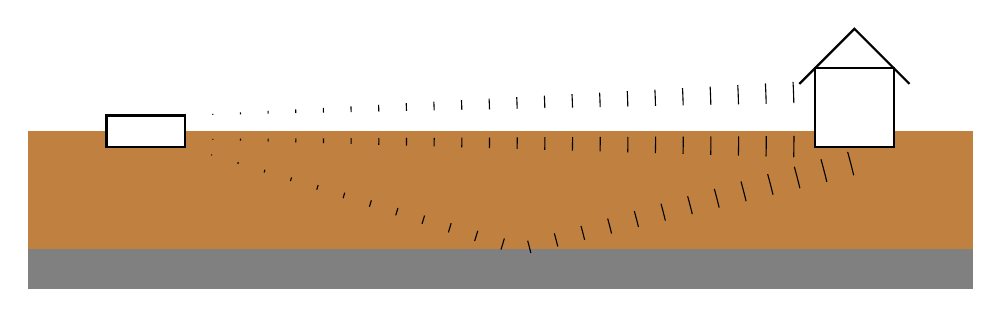
\begin{tikzpicture}
 \fill[color=brown] (-6,-1.5) rectangle (6, 0);
 \fill[color=gray] (-6,-2) rectangle (6,-1.5);
 \draw[thick, fill=white] (-5,-0.2)  rectangle (-4, 0.2);
 \draw[thick, fill=white] ( 4,-0.2)  rectangle ( 5, 0.8);
 \draw[thick] (3.8, 0.6) -- (4.5, 1.3) -- (5.2, 0.6);
 \draw[decorate,decoration={expanding waves, angle=1}] (-4, 0.2) -- (4, 0.5);
 \draw[decorate,decoration={expanding waves, angle=1}] (-4,-0.1) -- (4,-0.2);
 \draw[decorate,decoration={expanding waves, angle=1}] (-4,-0.2) -- (0.25,-1.5) -- (4.5,-0.4);
\end{tikzpicture}

\end{center}
\begin{description}[leftmargin=!,labelwidth=1mm]
\item[Quellen] Verkehr, Bauarbeiten, Maschinen, Naturereignisse
\item[Übertragungsweg] Boden (Dämpfung, Reflexion, Transmission) und Luft (hier nicht betrachtet) 
\item[Empfänger] Gebäude(teile), Lebewesen, Geräte
\end{description}
\end{frame}


\begin{frame}
\frametitle{Erschütterungsemission {\normalsize durch Verkehr}}

\only<1>{
Logarithmische Darstellung der Partikelgeschwindigkeit \cite{studer2008bodendynamik}
\begin{equation*}
 L_v=\mathrm{dB}(v)=20\log\left(\frac{v}{v_\mathrm{ref}}\right)
\end{equation*}
bezogen auf den Referenzwert $v_\mathrm{ref}=\SI{1e-6}{\milli\metre\per\second}$ (ISO 1683).
Damit folgende Übertragungsverluste und -verstärkungen
\begin{equation*}
L_\mathrm{immission}=L_\mathrm{emission}
\underbrace{-\Delta L_{v,\mathrm{geom}}-\Delta L_{v,\mathrm{mat}}- \Delta L_{v,\mathrm{refl}}}_{\text{Verluste im Übertragungsmedium}}
\underbrace{-\Delta L_{v,\mathrm{koppl}}-\Delta L_{v,\mathrm{empf}}}_{\text{Verluste/Verst. am Empfänger}}
\end{equation*}
}

\only<2>{
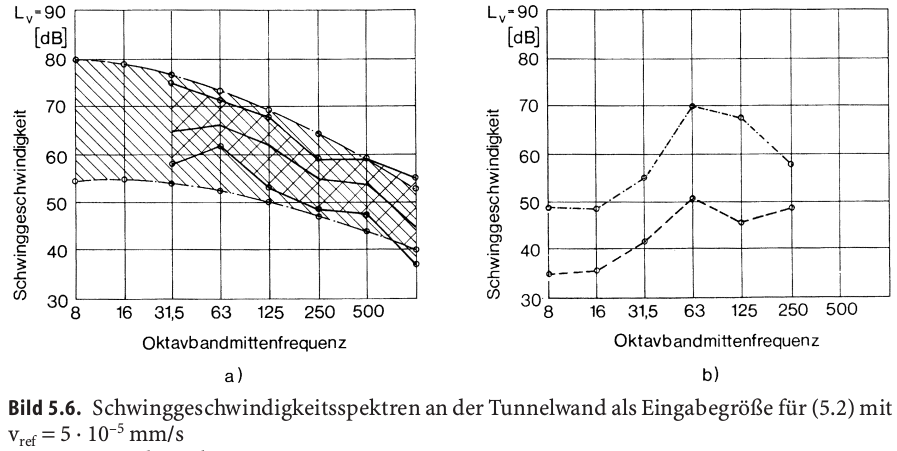
\includegraphics[width=\textwidth]{fig_img/tunnelspektrum} 
}
\end{frame}


\begin{frame}
\frametitle{Erschütterungsemission {\normalsize durch Bauarbeiten}}
Speziell für Spreng- und Rammerschütterungen \cite{studer2008bodendynamik} ist die Messung an der Quelle schwierig, deswegen wird die eingebrachte Energie als Kenngröße benutzt
\begin{equation*}
 v=cW^\alpha r^\beta.
\end{equation*}
\begin{description}
 \item[$v$] Partikelgeschwindigkeit
 \item[$c$] Koeffizient für Sprengstofftyp (experimentell bestimmt)
 \item[$W$] Sprengstoffgewicht
 \item[$\alpha$] Skalierungsfaktor ($\alpha\approx1/3$)
 \item[$r$] Abstand Quelle -- Empfänger
 \item[$\beta$] Skalierungsfaktor ($\beta=-2$ für Punktquelle)
\end{description}
Maschinen werden nach der gleichen Formel geschätzt \cite{studer2008bodendynamik}.
\end{frame}


\begin{frame}
\frametitle{Erschütterungseinwirkung} %TODO KB Wert
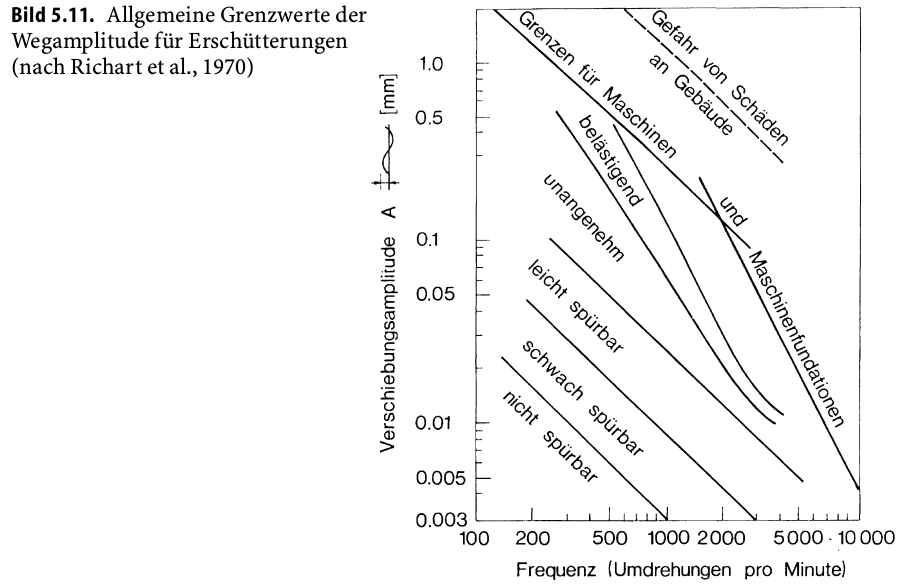
\includegraphics[width=0.88\textwidth]{fig_img/grenzwerte} 
%\cite{studer2008bodendynamik} % Belästigung (subjektiv) vor Schädigung
\end{frame}

\begin{frame}
\frametitle{Erschütterungseinwirkung {\normalsize auf Bauwerke}}
Länderspezifische Richtlinien (Deutschland: DIN 4150-3)

Richt- und Grenzwerte beziehen sich meist auf die Partikelgeschwindigkeit und werden unterteilt nach
\begin{description}
 \item[Häufigkeitsklassen]: gelegentlich, häufig, permanent
 \item[Empfindlichkeitsklassen]: sehr wenig, wenig, normal, erhöht empfindlich  
 \item[Frequenz]: $<\SI{30}{\hertz}$, $\SI{30}{\hertz}$--$\SI{60}{\hertz}$, $>\SI{60}{\hertz}$
\end{description}

\bigskip

Beispiel (nach SN 640312a) für häufige Vorgänge, normale Empfindlichkeit und eine Frequenz von $\SI{45}{\hertz}$ beträgt der Richtwert $v=\SI{8}{\milli\metre\per\second}$.
\end{frame}


\begin{frame}
\frametitle{Erschütterungseinwirkung {\normalsize auf Menschen}}
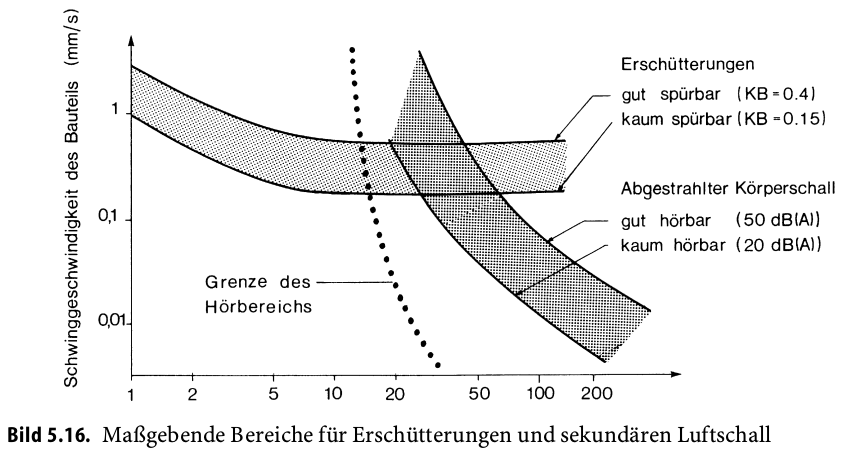
\includegraphics[width=0.99\textwidth]{fig_img/grenzwerte_schall} 
\end{frame}


%\begin{frame}
%\frametitle{Erschütterungseinwirkung{\normalsize auf Geräte}}
%ISO 8569:1996 Mechanical vibration and shock – Measurement and evaluation of
%shock and vibration effects on sensitive equipment in buildings
%\cite{studer2008bodendynamik}
%\end{frame}


\begin{frame}
\frametitle{Erschütterungsreduktion}
\begin{description}
 \item[Quelle:] optimiertes Sprengschema, Maschinenfundamente, Unterschottermatten, Zusatzmassen
 
 \item[Übertragungsmedium:] 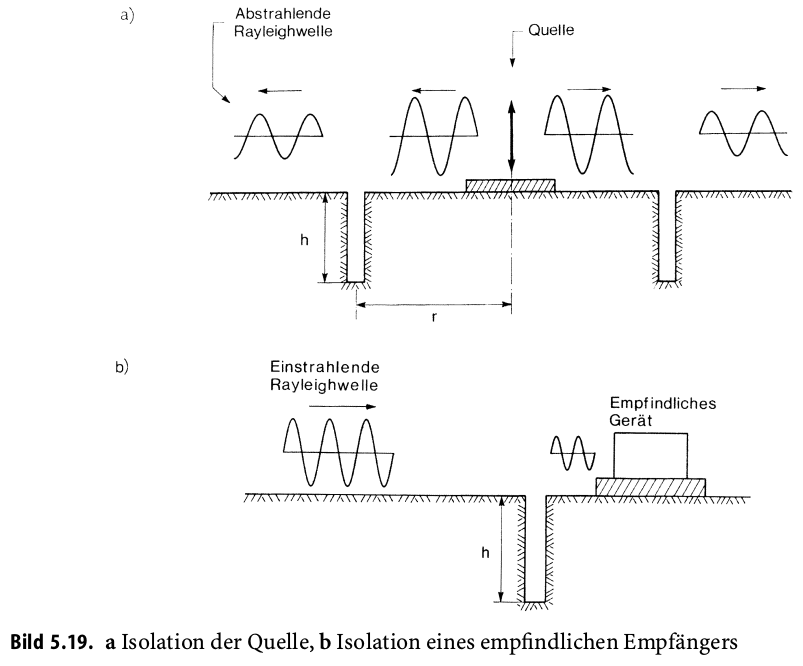
\includegraphics[width=0.49\textwidth]{fig_img/schlitz}
 
 \item[Empfänger:] Auflagerung/Fundament, Schwingungstilger 
\end{description}
\end{frame}


\begin{frame}
\frametitle{Beispiel}

\only<1>{
\begin{figure}
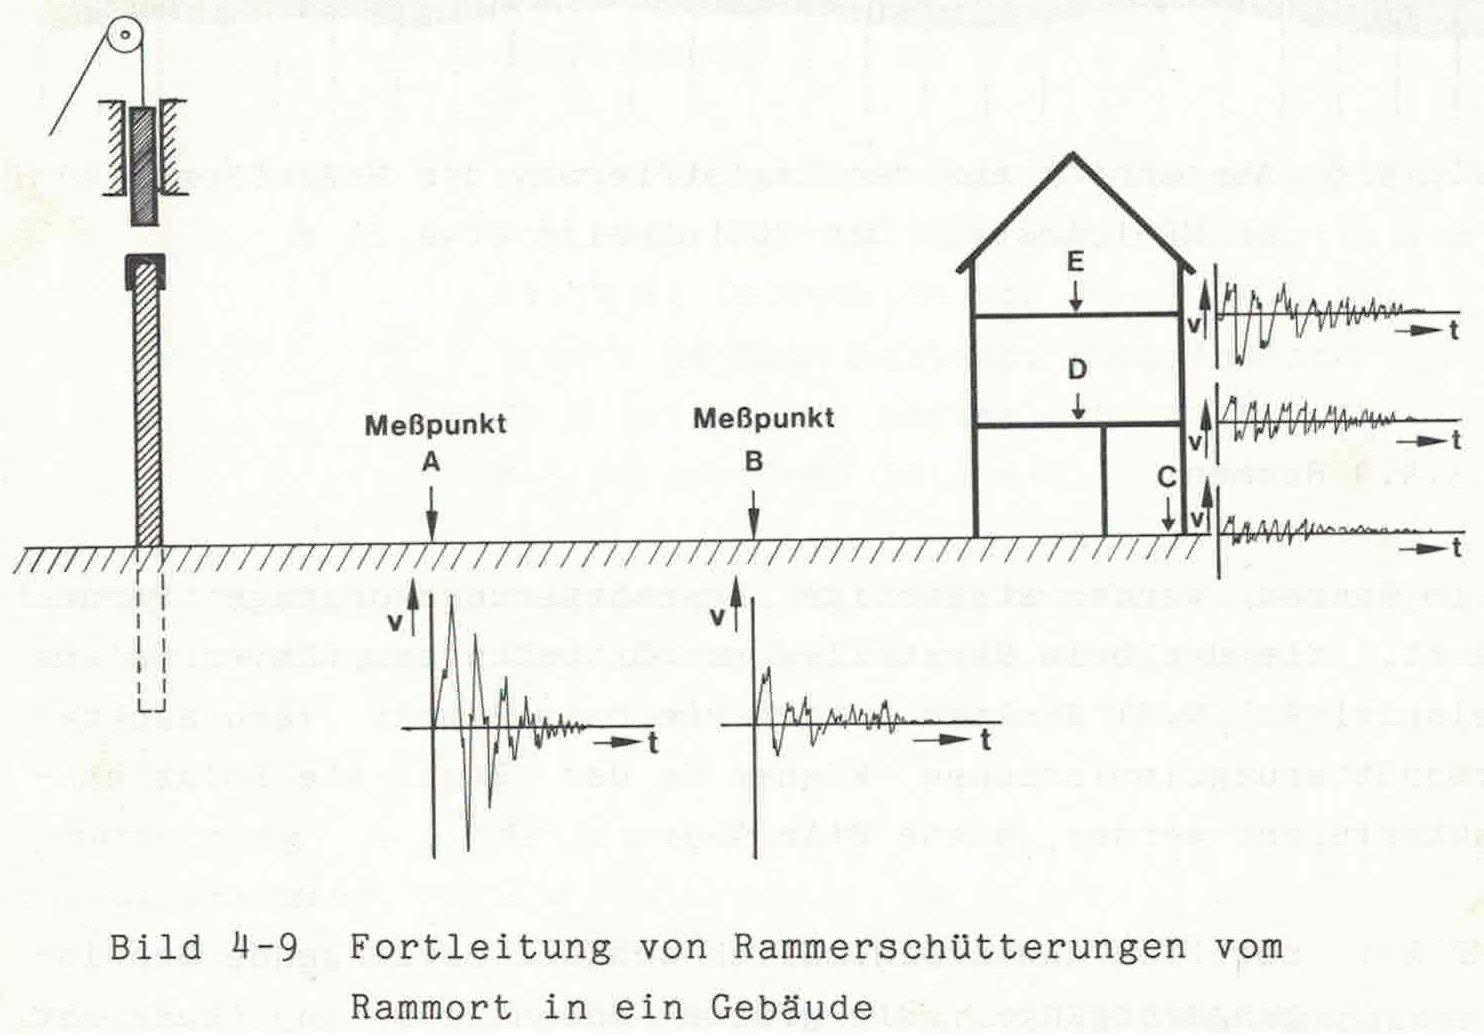
\includegraphics[width=0.7\textwidth]{fig_img/beispiel_ramme} 
\caption*{Messpunktanordnung \cite{haupt1986bodendynamik}}
\end{figure}
}%only

\only<2>{
\begin{figure}
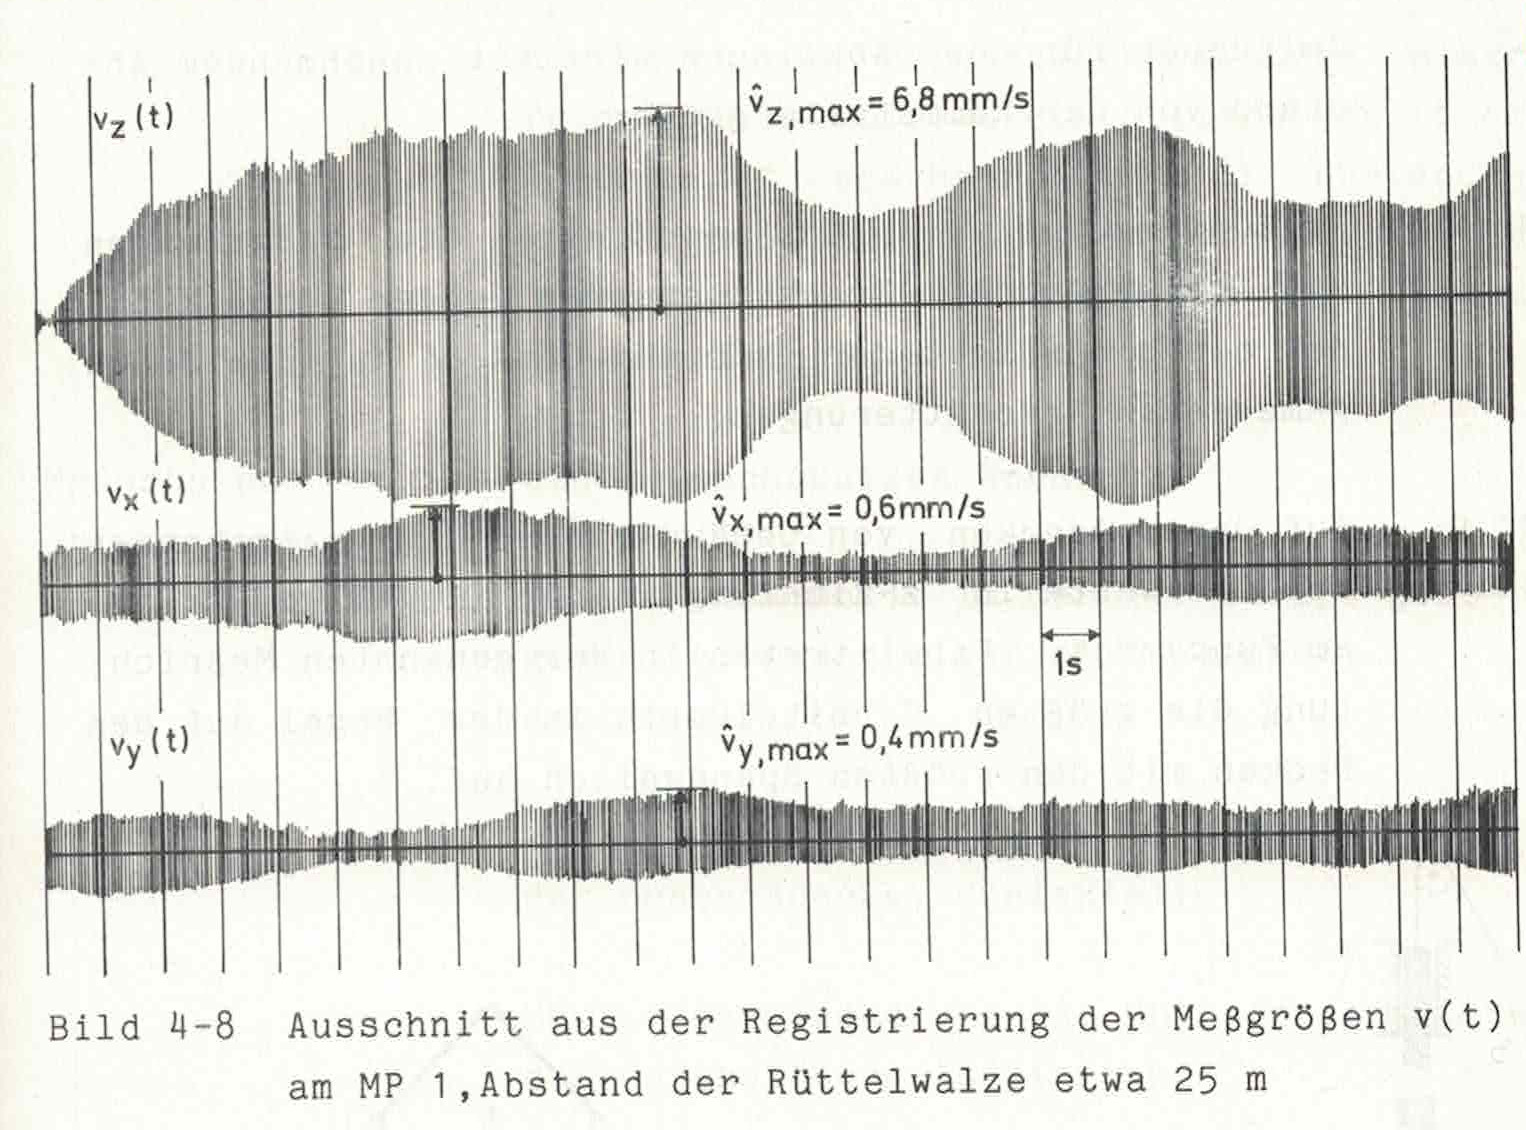
\includegraphics[width=0.66\textwidth]{fig_img/beispiel_ruettelwalze} 
\caption*{Geschwindigkeitsignal in drei Raumrichtungen \cite{haupt1986bodendynamik}}
\end{figure}
}%only

\end{frame}




\subsection{Erdbebensicheres Bauen}

\begin{frame}
\frametitle{Historie und Spannungskarte}
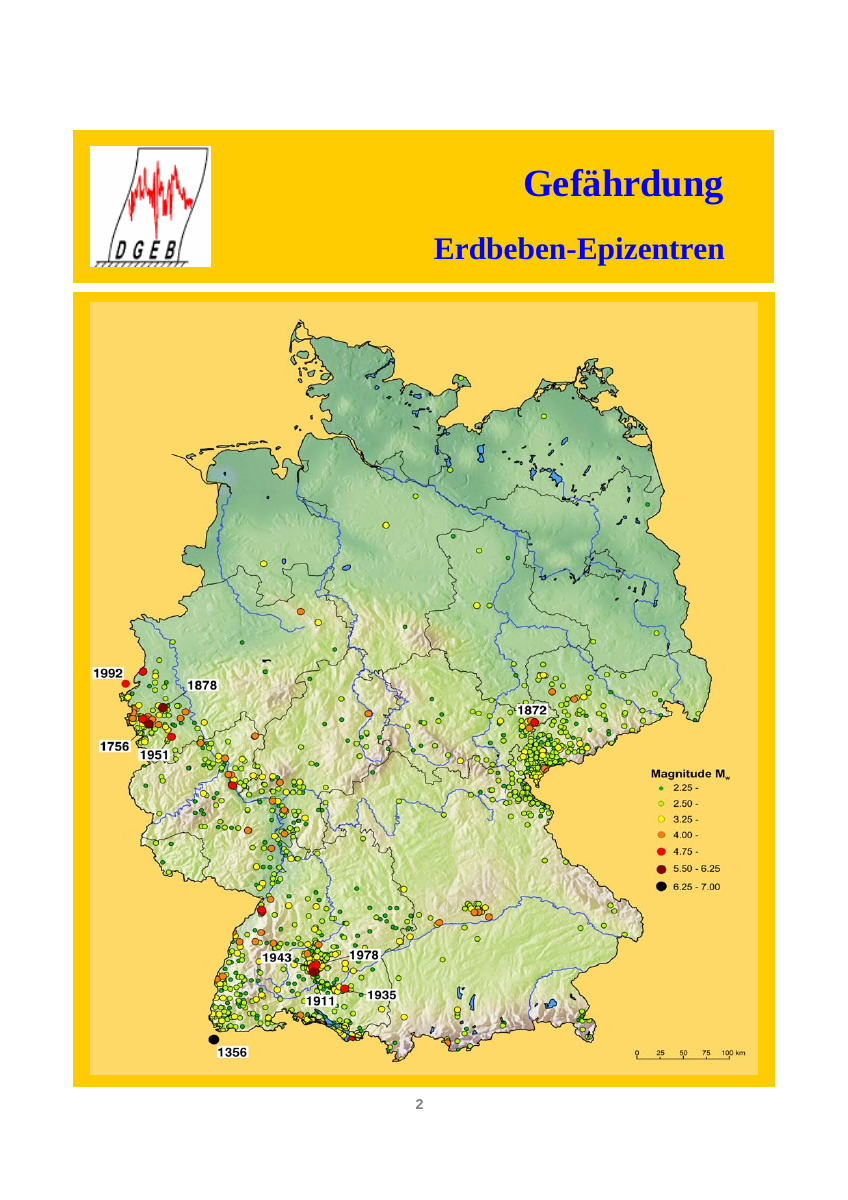
\includegraphics[width=0.43\textwidth]{fig_img/erdbeben_de} %TODO cite DGEB
\hfill
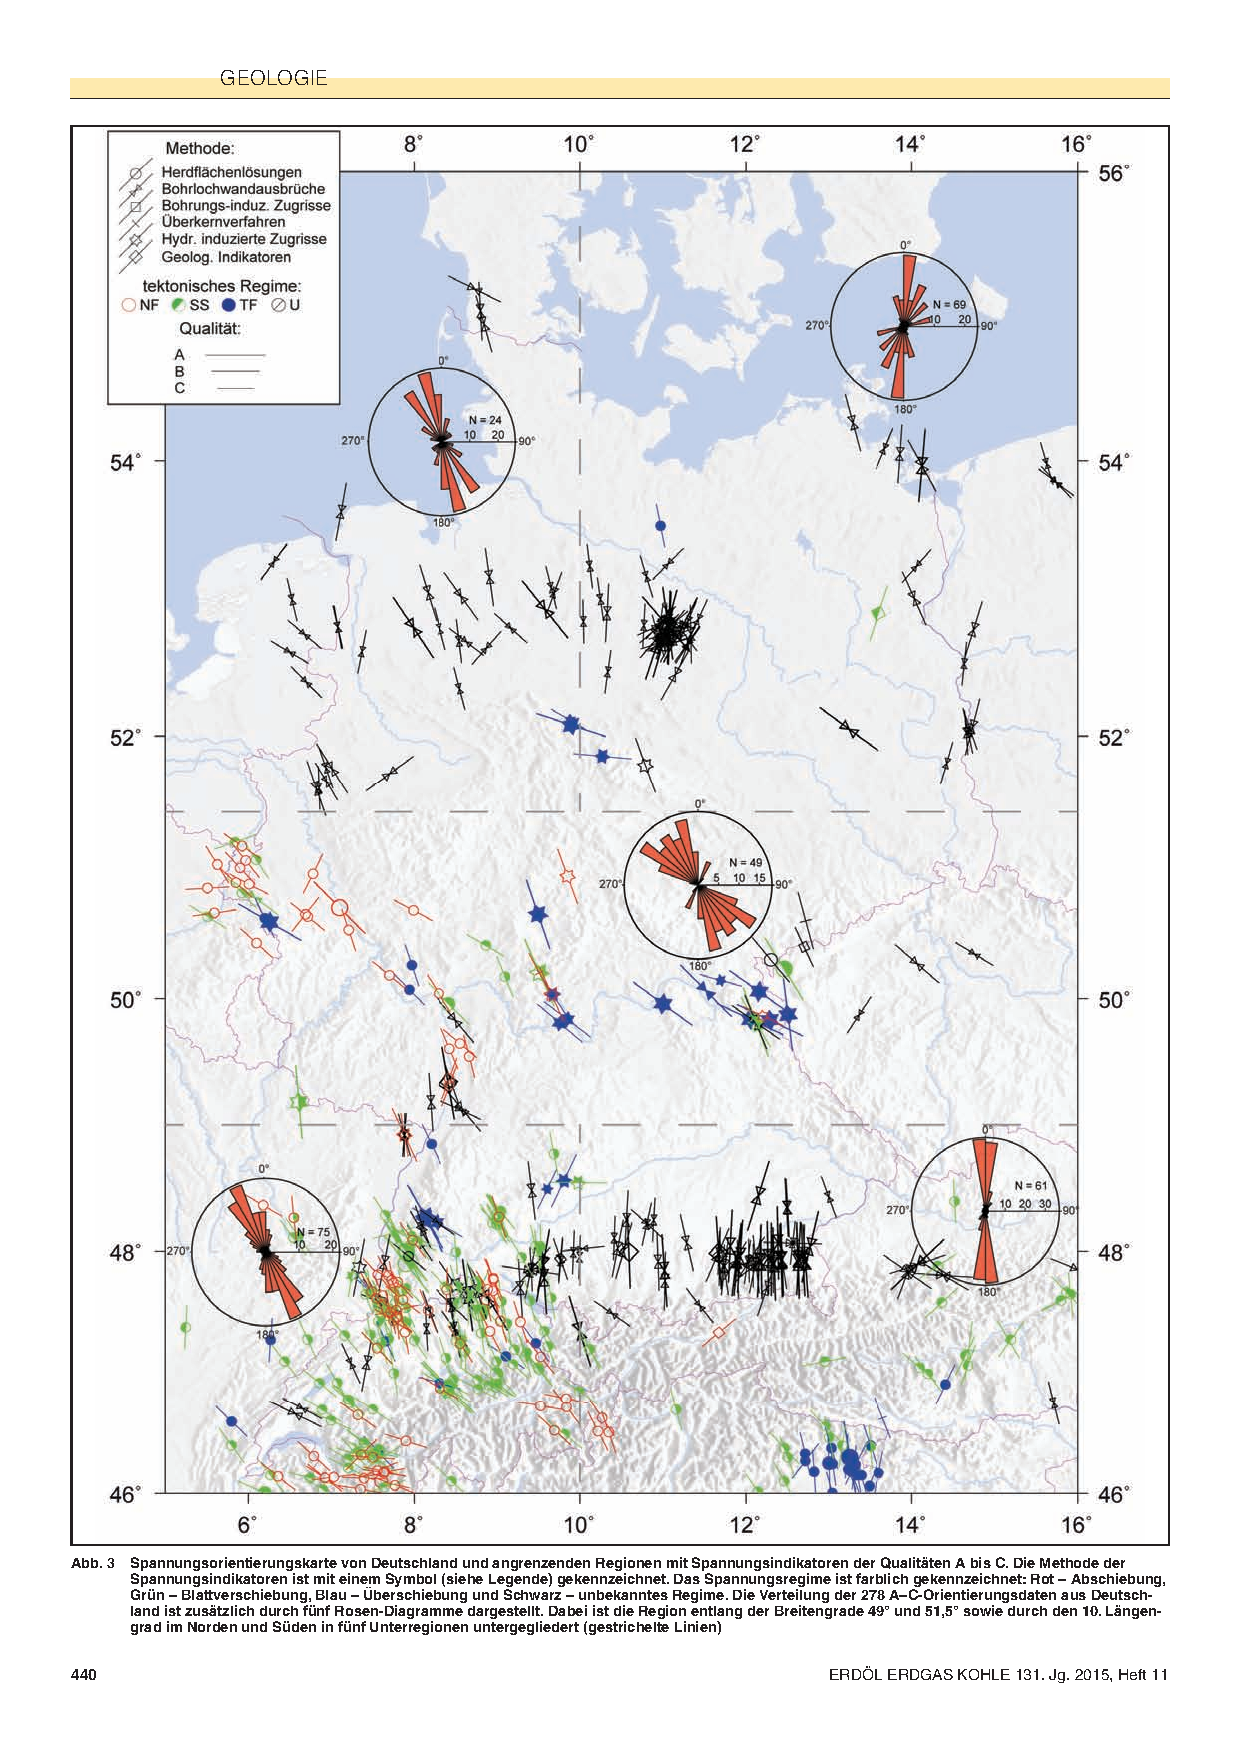
\includegraphics[width=0.4\textwidth]{fig_pdf/spannungslandkarte} %TODO stress map
\end{frame}


\begin{frame}
\frametitle{Effekte}
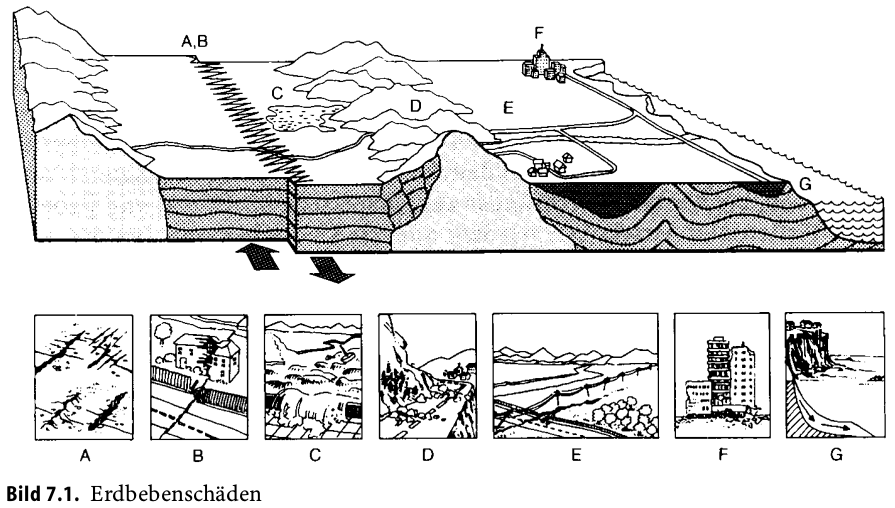
\includegraphics[width=0.95\textwidth]{fig_img/erdbebenschaeden} %TODO cite Studer
\end{frame}


\begin{frame}
\frametitle{Entstehung}
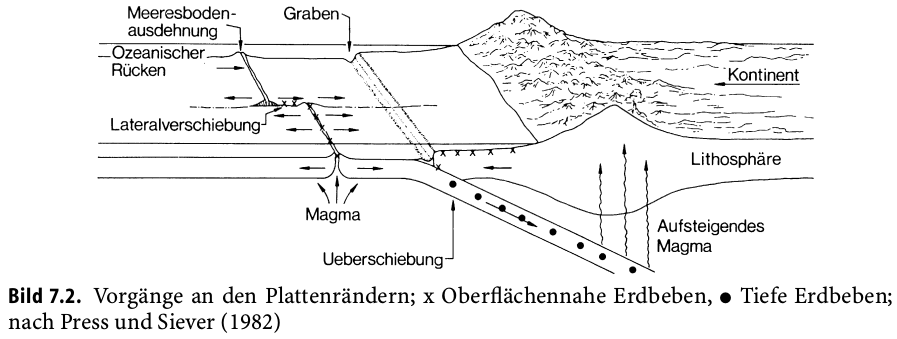
\includegraphics[width=\textwidth]{fig_img/plattenraender} %TODO cite Studer
\end{frame}


\begin{frame}
\frametitle{Verwerfungstypen}
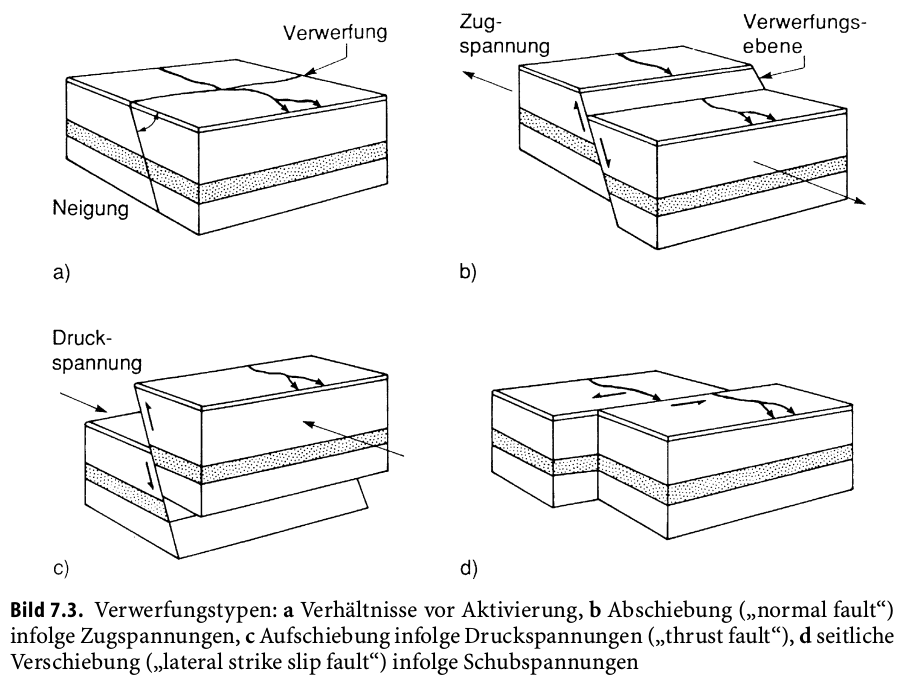
\includegraphics[width=0.72\textwidth]{fig_img/verwerfungstypen} %TODO cite Studer
\end{frame}


\begin{frame}
\frametitle{Geometrie}
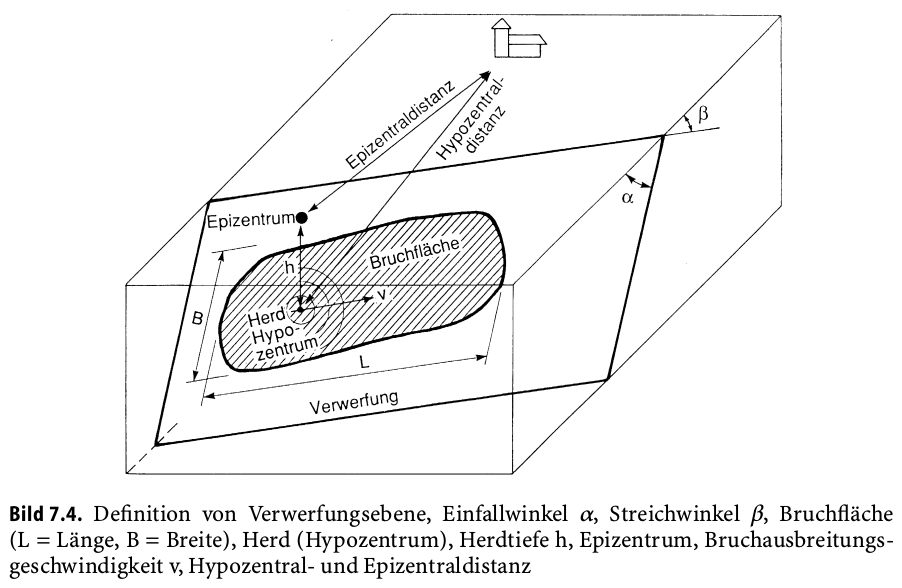
\includegraphics[width=0.83\textwidth]{fig_img/erdbebengeometrie} %TODO cite Studer
\end{frame}


\begin{frame}
\frametitle{Beschreibung}
\textbf{Intensität:} Phänomenologische Beschreibung nach hervorgerufener Wirkung\\
1 (nicht fühlbar) \dots 6 (Gebäudeschäden) \dots 12 (vollständig verwüstend) Klassifzierung nach EMS-1998

\bigskip

\textbf{Magnitude:} Maß für die freigesetzte Energie
\begin{itemize}
 \item Richter $M_\mathrm{L} = \log_{10}\left(\dfrac{\mathrm{max}(u_{\SI{100}{\kilo\metre}})}{u_\mathrm{ref}} \right)$ bezogen auf Referenzpunkt  % +1 entspricht Energie 31.6, Verschiebung 10 [Richter]
 \item Moment  $M_\mathrm{W}=\frac{2}{3}\log_{10}(M_0) - 6$  bezogen auf Erdbebenherd $M_0 = \mu A \Delta u$ $[M_0]=\SI{}{\newton\metre}$, mit Scherfestigkeit $\mu$ an der Bruchzone, Bruchfläche $A$ und mittlerer Verschiebung $\Delta u$  % [ToDo]
\end{itemize}
\end{frame}


\begin{frame}
\frametitle{Vorgehenskonzepte}
\begin{description}
 \item[deterministisch] sehr spezifisch (Ort, Szenario), modellbasiert (Quelle, Übertagungsmedium, Empfänger), Problem Parameterbestimmung
 
 \item[probabilistisch] ausgehend von bisherigen räumlichen und zeitlichen Verläufen werden erdenkliche Erdbeben mit Wahrscheinlichkeiten versehen.
\end{description}

\vfill

Bewertung hinsichtlich
\begin{itemize}
 \item Baugrunderschütterung
 \item Bodenverflüssigung
 \item Hangrutschungen
 \item Risse an der Erdoberfläche
\end{itemize}


\end{frame}


\begin{frame}
\frametitle{Berücksichtigung in der Auslegung}
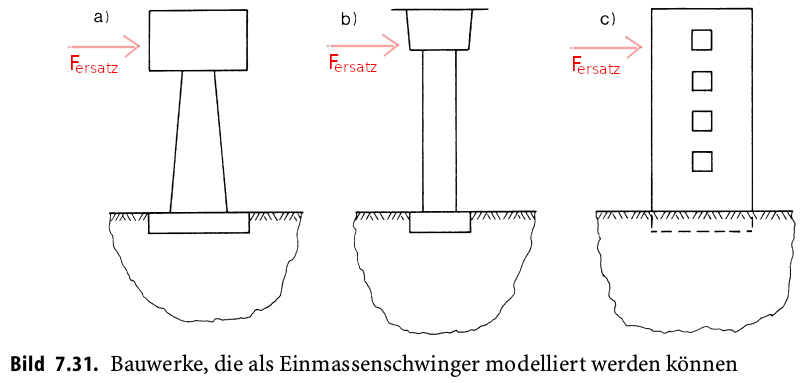
\includegraphics[width=\textwidth]{fig_img/einmassenmodell_erdbeben}

%Idee: Bauwerke (oder einzelne Schwingformen) lassen sich durch Einmassenschwinger annähern
\end{frame}


\begin{frame}
\frametitle{Antwortspektrum}  % allgemein/standortspezifisch
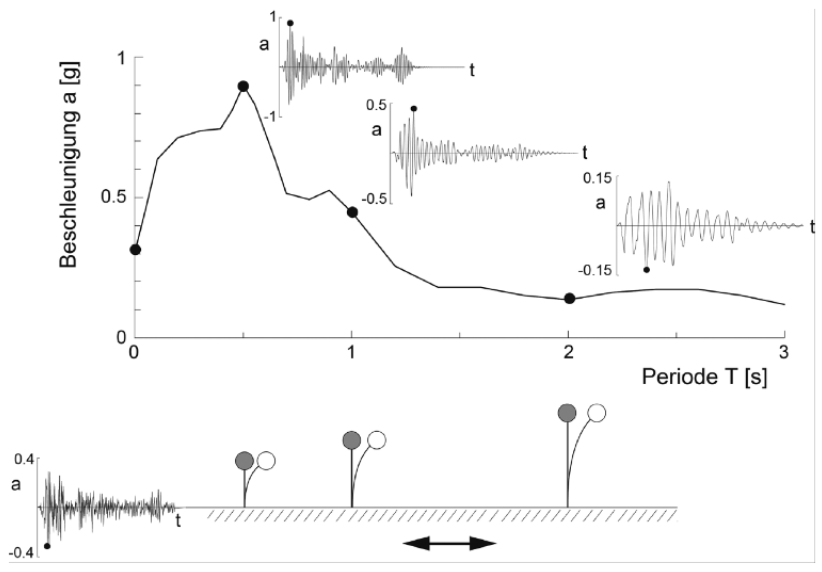
\includegraphics[width=0.77\textwidth]{fig_img/antwortspektrum} %TODO cite Vrettos
\end{frame}


\begin{frame}
\frametitle{Bemessungsspektrum}  % allgemein/standortspezifisch
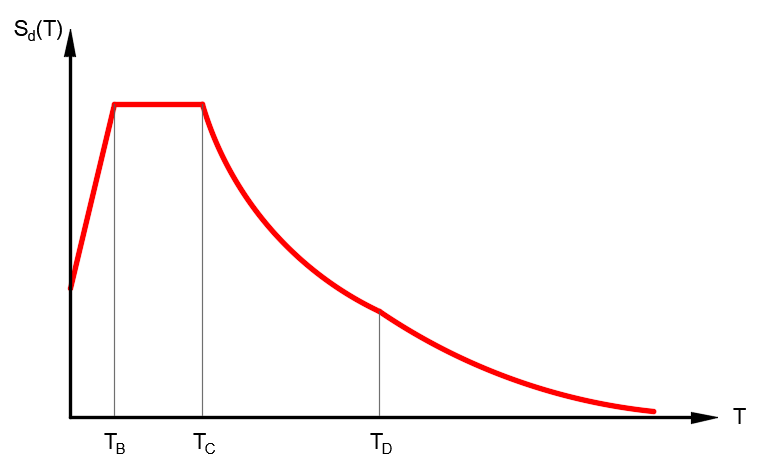
\includegraphics[width=0.75\textwidth]{fig_img/bemessungsspektrum} %TODO cite

Das Bemessungsspektrum ist ein ``geglättetes'' und ``informationsangereichertes'' Antwortspektrum. 
\end{frame}

\begin{frame}
\frametitle{Auslegung {\normalsize anhand des Bemessungspektrums}}  % allgemein/standortspezifisch 
\only<1>{
\begin{align*}
0<T\le T_\mathrm{B}  &: \quad S_\mathrm{d}(T)=a_\mathrm{gR} \gamma_l S \left[ 1+\frac{T}{T_\mathrm{B}}\left(\frac{2.5}{q}-1\right) \right] \\
T_\mathrm{B}<T\le T_\mathrm{C}  &: \quad S_\mathrm{d}(T)=a_\mathrm{gR} \gamma_l S \frac{2.5}{q}\\
T_\mathrm{C}<T\le T_\mathrm{D}  &: \quad S_\mathrm{d}(T)=a_\mathrm{gR} \gamma_l S \frac{2.5}{q}\frac{T_\mathrm{C}}{T}\\
T_\mathrm{D}<T\le \SI{4}{\second}  &: \quad S_\mathrm{d}(T)=a_\mathrm{gR} \gamma_l S \frac{2.5}{q}\frac{T_\mathrm{C} T_\mathrm{D}}{T^2}
\end{align*}
$T$ ist die Periodendauer des Einmassenschwingers, alle übrigen Parameter charakterisieren das Erdbebengebiet, den Baugrund und das Bauwerk.
}%only

\only<2>{
$S_\mathrm{d}$ entspricht einer Beschleunigung, demzufolge berechnet sich die Ersatzkraft
\begin{equation*}
 F_\mathrm{ersatz} = S_d(T) m \lambda,
\end{equation*}
wobei $\lambda$ ein Korrekturwert für die Stockwerke ist.

\vfill

Die Periode eines Gebäudes kann in Abhängigkeit der Höhe $h$ geschätzt werden
\begin{equation*}
 T = C_t h^{3/4}
\end{equation*}
wobei $C_t$ das Tragwerk charakterisiert ($C_t=\SI{0.085}{}$ für biegesteife räumliche Stahlrahmen, $C_t=\SI{0.075}{}$ für biegesteife räumliche Stahlbetonrahmen und $C_t=\SI{0.050}{}$ für andere Rahmen).

}%


\end{frame}




\begin{frame}
\frametitle{Konstruktionshinweise}  % allgemein/standortspezifisch
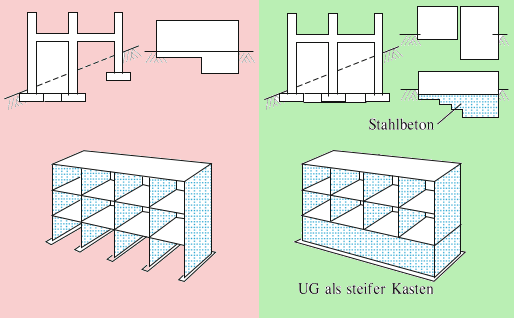
\includegraphics[width=0.495\textwidth]{fig_img/erdbebensicher_konstruieren1} 
\hfill
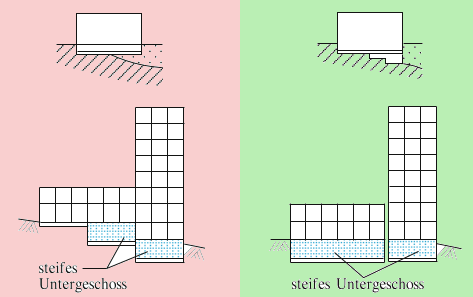
\includegraphics[width=0.495\textwidth]{fig_img/erdbebensicher_konstruieren2} 
\cite{Schmidt2017}
\end{frame}



%%%%%%%%%%%%%%%%%%%%%%%%%%%%%%%%%%%%%%%%%%%%%%%%

\section*{Literaturverzeichnis}

\begin{frame}[allowframebreaks]{}
	\printbibliography
\end{frame}
\end{document}
